Pada konfigurasi \textit{baseline} (S1--S4), APFPlanner menggunakan parameter navigasi yang bersifat tetap untuk menentukan kecepatan pergerakan robot dan kekuatan gaya tolak terhadap obstacle. Pendekatan tersebut relatif sederhana dan memiliki kompleksitas komputasi yang rendah, namun kurang mampu beradaptasi terhadap perubahan kondisi lingkungan yang terjadi secara dinamis. Ketika robot memasuki area dengan obstacle yang rapat atau traversability lingkungan menurun, penggunaan parameter tetap dapat menghasilkan perilaku navigasi yang terlalu agresif maupun terlalu konservatif.

Untuk mengatasi keterbatasan tersebut, penelitian ini mengintegrasikan logika fuzzy Mamdani sebagai mekanisme adaptasi parameter navigasi. Berbeda dengan pendekatan yang menggunakan fuzzy sebagai pengendali utama robot, sistem fuzzy pada penelitian ini berperan sebagai lapisan adaptif (\textit{adaptive layer}) yang memodifikasi parameter APF berdasarkan kondisi lingkungan yang diamati sensor. Pendekatan serupa telah banyak digunakan pada sistem navigasi robot bergerak karena mampu meningkatkan fleksibilitas pengambilan keputusan tanpa menambah kompleksitas komputasi secara signifikan (\cite{Haider2022,Benaicha2026}).

Masukan sistem fuzzy terdiri atas jarak obstacle terdekat ($d_{obs}$) yang diperoleh dari data LiDAR dan nilai traversability efektif ($\tau_{eff}$) hasil fusi sensor. Berdasarkan kedua informasi tersebut, sistem menghasilkan dua parameter adaptif, yaitu \textit{speed scale} ($S$) dan \textit{repulsive gain} ($G$), yang selanjutnya digunakan untuk menyesuaikan perilaku APFPlanner secara \textit{real-time}.

\subsection{Variabel Input dan Output}

Variabel masukan pertama adalah jarak obstacle terdekat ($d_{obs}$) yang diperoleh dari hasil pemrosesan LiDAR sebagaimana dijelaskan pada Subbab~\ref{sec:pemrosesan_lidar}. Variabel ini digunakan untuk merepresentasikan tingkat kedekatan robot terhadap obstacle yang berada di sekitarnya.

Variabel masukan kedua adalah traversability efektif ($\tau_{eff}$) yang diperoleh melalui meka\-nisme fusi sensor pada Subbab~\ref{sec:fusi_traversability}. Nilai tersebut menggambarkan tingkat keamanan area yang berada di depan robot berdasarkan informasi geometris dan termal.

Sementara itu, sistem fuzzy menghasilkan dua variabel keluaran, yaitu:

\begin{enumerate}
\item \textit{Speed Scale} ($S$), yang digunakan untuk mengatur kecepatan linear robot.
\item \textit{Repulsive Gain} ($G$), yang digunakan untuk mengatur kekuatan gaya tolak obstacle pada APF.
\end{enumerate}

Tabel~\ref{tab:variabel_fuzzy} menunjukkan rentang setiap variabel yang digunakan dalam sistem fuzzy.

\begin{table}[H]
\centering
\caption{Variabel masukan dan keluaran sistem fuzzy}
\label{tab:variabel_fuzzy}
\begin{tabular}{llll}
\toprule
\textbf{Variabel} &
\textbf{Simbol} &
\textbf{Jenis} &
\textbf{Rentang} \\
\midrule
Jarak obstacle &
$d_{obs}$ &
Masukan &
0 -- 6 m \\

Traversability efektif &
$\tau_{eff}$ &
Masukan &
0 -- 1 \\

Speed Scale &
$S$ &
Keluaran &
0 -- 1 \\

Repulsive Gain &
$G$ &
Keluaran &
0 -- 1 \\
\bottomrule
\end{tabular}
\end{table}

% \subsection{Fungsi Keanggotaan}
% \label{sec:fungsi_keanggotaan}

% Setiap variabel fuzzy direpresentasikan menggunakan fungsi keanggotaan berbentuk segitiga dan trapesium. Bentuk fungsi tersebut dipilih karena sederhana, mudah diimplementasikan, serta mampu merepresentasikan perubahan kondisi lingkungan secara bertahap (\cite{Mamdani1974}).

% \subsubsection{Fungsi Keanggotaan Jarak Obstacle}

% Variabel jarak obstacle ($d_{obs}$) dibagi menjadi tiga himpunan linguistik, yaitu:

% \begin{enumerate}
% \item \textit{Near}
% \item \textit{Medium}
% \item \textit{Far}
% \end{enumerate}

% Fungsi keanggotaan yang digunakan ditunjukkan pada Gambar~\ref{fig:mf_jarak}.

% \begin{figure}[H]
% \centering
% 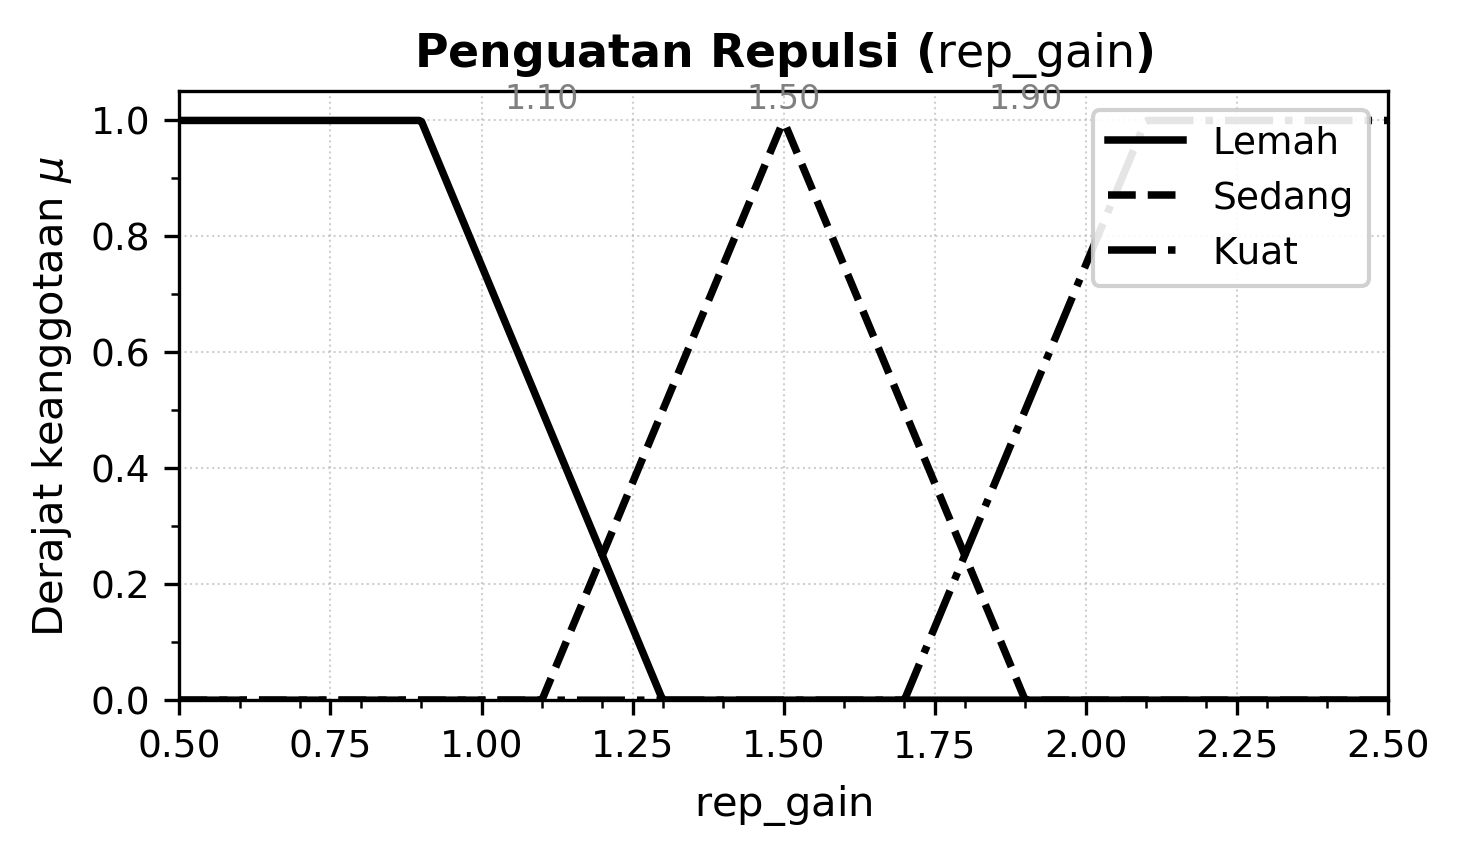
\includegraphics[width=0.8\textwidth]{gambar/3.7_fig_mf_gain.png}
% \caption{Fungsi keanggotaan variabel jarak obstacle.}
% \label{fig:mf_jarak}
% \end{figure}

% \subsubsection{Fungsi Keanggotaan Traversability}

% Variabel traversability efektif ($\tau_{eff}$) dibagi menjadi tiga himpunan linguistik, yaitu:

% \begin{enumerate}
% \item \textit{Low}
% \item \textit{Medium}
% \item \textit{High}
% \end{enumerate}

% Fungsi keanggotaan traversability ditunjukkan pada Gambar~\ref{fig:mf_traversability}.

% \begin{figure}[H]
% \centering
% 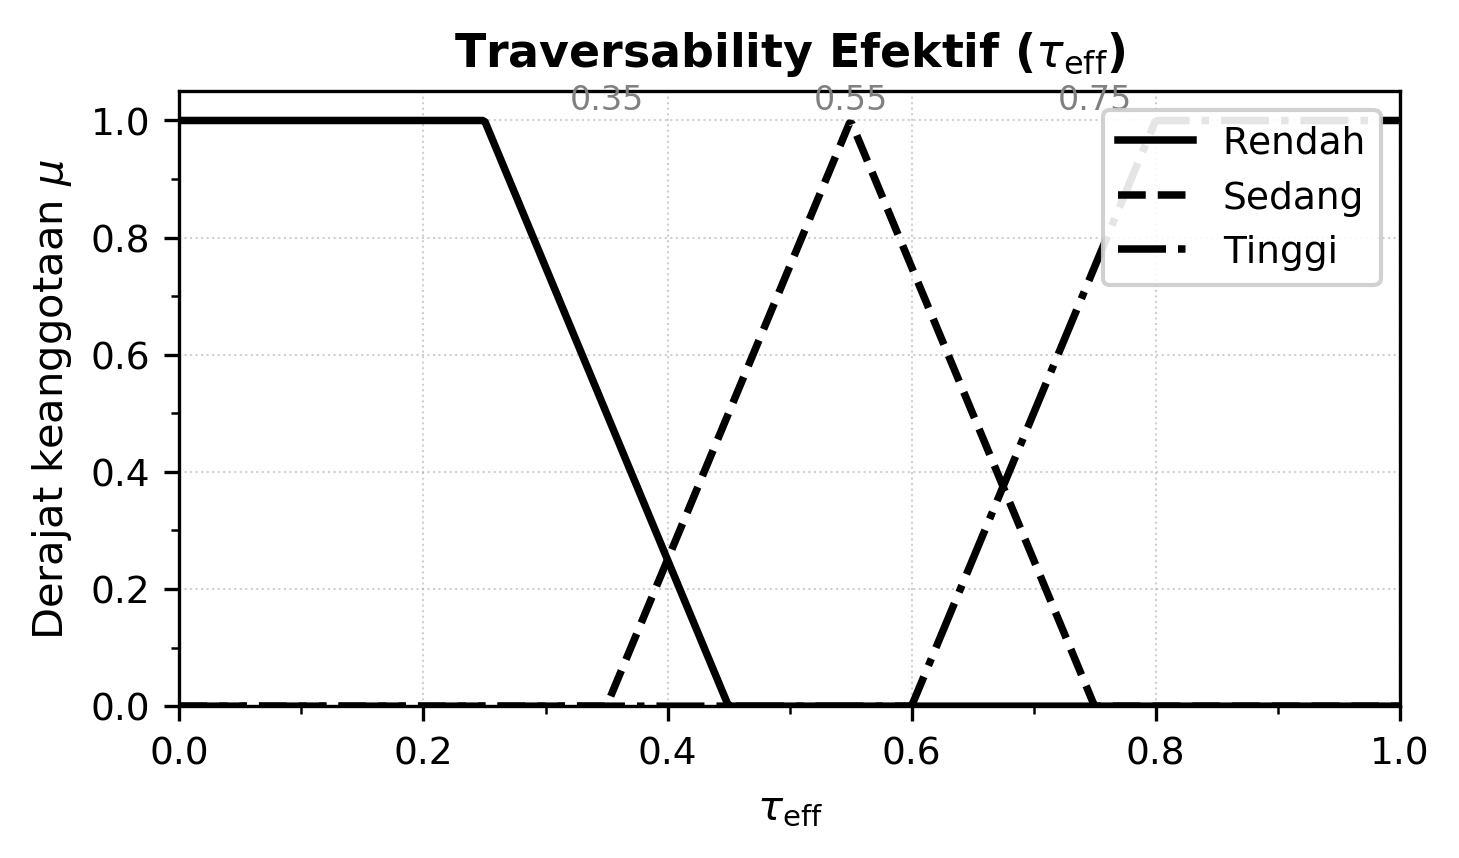
\includegraphics[width=0.8\textwidth]{gambar/3.7_fig_mf_trav.png}
% \caption{Fungsi keanggotaan variabel traversability efektif.}
% \label{fig:mf_traversability}
% \end{figure}

% \subsubsection{Fungsi Keanggotaan Speed Scale}

% Variabel keluaran \textit{Speed Scale} dibagi menjadi tiga himpunan linguistik:

% \begin{enumerate}
% \item \textit{Slow}
% \item \textit{Medium}
% \item \textit{Fast}
% \end{enumerate}

% Fungsi keanggotaan ditunjukkan pada Gambar~\ref{fig:mf_kecepatan}.

% \begin{figure}[H]
% \centering
% 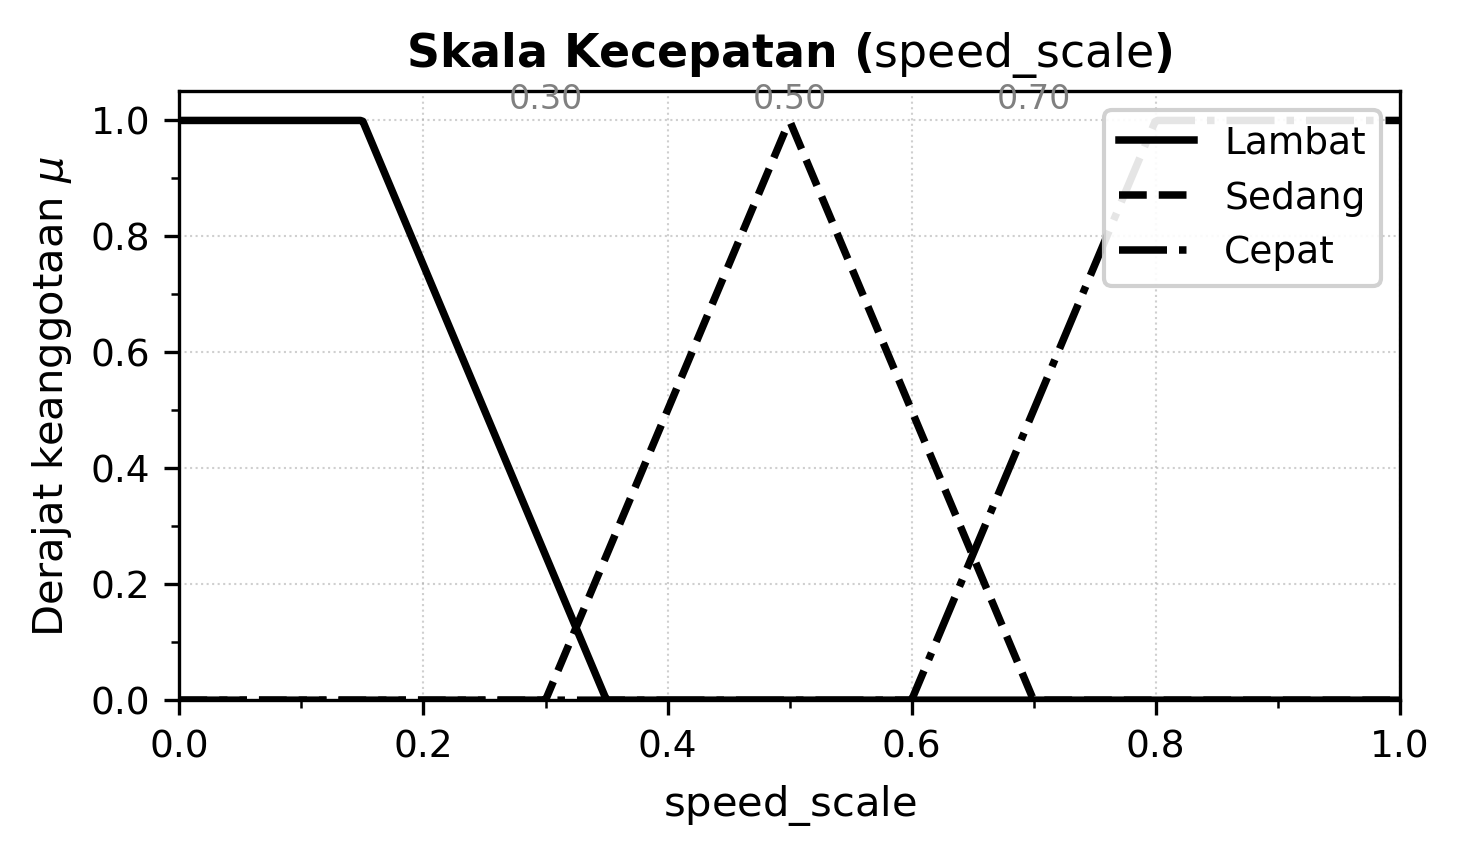
\includegraphics[width=0.8\textwidth]{gambar/3.7_fig_mf_kecepatan.png}
% \caption{Fungsi keanggotaan variabel \textit{Speed Scale}.}
% \label{fig:mf_kecepatan}
% \end{figure}

% \subsubsection{Fungsi Keanggotaan Repulsive Gain}

% Variabel keluaran \textit{Repulsive Gain} dibagi menjadi tiga himpunan linguistik:

% \begin{enumerate}
% \item \textit{Weak}
% \item \textit{Medium}
% \item \textit{Strong}
% \end{enumerate}

% Fungsi keanggotaan ditunjukkan pada Gambar~\ref{fig:mf_gain}.

% \begin{figure}[H]
% \centering
% 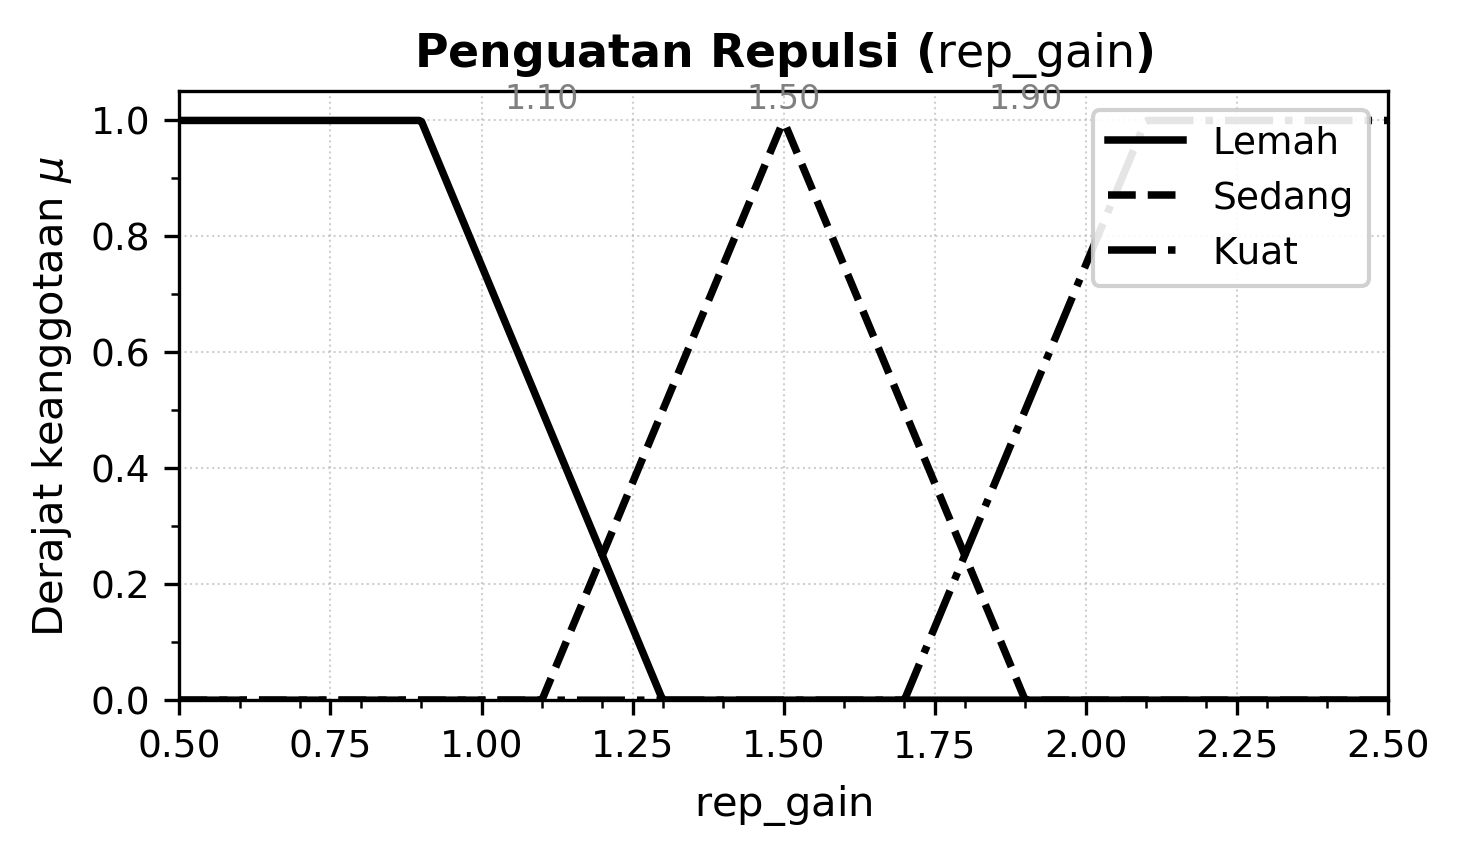
\includegraphics[width=0.8\textwidth]{gambar/3.7_fig_mf_gain.png}
% \caption{Fungsi keanggotaan variabel \textit{Repulsive Gain}.}
% \label{fig:mf_gain}
% \end{figure}

\subsection{Fungsi Keanggotaan}
\label{sec:fuzzy_mf}
% -----------------------------------------------------------------------

Setiap variabel fuzzy didefinisikan menggunakan tiga label linguistik dengan fungsi keanggotaan berbentuk trapesium (\textit{trapmf}) atau segitiga (\textit{trimf}). Bentuk trapesium dipilih untuk label ujung (rendah/lambat/lemah dan tinggi/cepat/kuat) karena memberikan respons jenuh (\textit{saturation}) di area ekstrem, sehingga nilai input yang sangat ekstrem selalu mendapatkan keanggotaan penuh pada label tersebut~\cite{Benaicha2026}. Bentuk segitiga dipilih untuk label tengah karena memberikan transisi yang halus dan simetris.

Fungsi keanggotaan didefinisikan sebagai berikut. Untuk fungsi segitiga:
\begin{equation}
    \mu_\text{trimf}(x;\,a,b,c) =
    \begin{cases}
        0 & x \leq a \\
        \dfrac{x - a}{b - a} & a < x \leq b \\[6pt]
        \dfrac{c - x}{c - b} & b < x \leq c \\
        0 & x > c
    \end{cases}
    \label{eq:trimf}
\end{equation}
dan untuk fungsi trapesium:
\begin{equation}
    \mu_\text{trapmf}(x;\,a,b,c,d) =
    \begin{cases}
        0 & x \leq a \\
        \dfrac{x - a}{b - a} & a < x \leq b \\[4pt]
        1 & b < x \leq c \\[4pt]
        \dfrac{d - x}{d - c} & c < x \leq d \\
        0 & x > d
    \end{cases}
    \label{eq:trapmf}
\end{equation}
Kasus khusus $a = b$ (tepi naik vertikal) atau $c = d$ (tepi turun vertikal) ditangani sebagai nilai langsung 1 atau 0 pada titik tersebut, konsisten dengan implementasi \texttt{skfuzzy.trapmf}.

\subsubsection*{a. Fungsi Keanggotaan Input: Jarak \textit{Obstacle} ($d_\text{obs}$)}

Input jarak didefinisikan dengan tiga label pada domain $[0{,}0,\ 2{,}0]$~m:
\begin{align}
    \mu_\text{dekat}(d)  &= \mu_\text{trapmf}(d;\;0{,}00,\;0{,}00,\;0{,}30,\;0{,}60) \label{eq:mf_dekat} \\
    \mu_\text{sedang}(d) &= \mu_\text{trimf}(d;\;0{,}40,\;0{,}80,\;1{,}20)           \label{eq:mf_sedang_d} \\
    \mu_\text{jauh}(d)   &= \mu_\text{trapmf}(d;\;1{,}00,\;1{,}40,\;2{,}00,\;2{,}00) \label{eq:mf_jauh}
\end{align}
Label \textit{Dekat} memiliki keanggotaan penuh untuk jarak $d \leq 0{,}30$~m dan menurun hingga nol pada $d = 0{,}60$~m. Label \textit{Jauh} mulai naik dari $d = 1{,}00$~m dan mencapai keanggotaan penuh pada $d \geq 1{,}40$~m.

\subsubsection*{b. Fungsi Keanggotaan Input: Traversability ($\tau_\text{eff}$)}

Input traversability didefinisikan dengan tiga label pada domain $[0{,}0,\ 1{,}0]$:
\begin{align}
    \mu_\text{rendah}(\tau) &= \mu_\text{trapmf}(\tau;\;0{,}00,\;0{,}00,\;0{,}25,\;0{,}45) \label{eq:mf_rendah} \\
    \mu_\text{sedang}(\tau) &= \mu_\text{trimf}(\tau;\;0{,}35,\;0{,}55,\;0{,}75)           \label{eq:mf_sedang_t} \\
    \mu_\text{tinggi}(\tau) &= \mu_\text{trapmf}(\tau;\;0{,}60,\;0{,}80,\;1{,}00,\;1{,}00) \label{eq:mf_tinggi}
\end{align}
Label \textit{Rendah} mencakup kondisi ketika jalur banyak terhalang \textit{obstacle} termal atau koridor sempit. Label \textit{Tinggi} mencakup kondisi jalur bebas dan koridor lebar.

\subsubsection*{c. Fungsi Keanggotaan Output: Skala Kecepatan}

Output kecepatan didefinisikan dengan tiga label pada domain $[0{,}0,\ 1{,}0]$:
\begin{align}
    \mu_\text{lambat}(s) &= \mu_\text{trapmf}(s;\;0{,}00,\;0{,}00,\;0{,}15,\;0{,}35) \label{eq:mf_lambat} \\
    \mu_\text{sedang}(s) &= \mu_\text{trimf}(s;\;0{,}30,\;0{,}50,\;0{,}70)           \label{eq:mf_sedang_s} \\
    \mu_\text{cepat}(s)  &= \mu_\text{trapmf}(s;\;0{,}60,\;0{,}80,\;1{,}00,\;1{,}00) \label{eq:mf_cepat}
\end{align}

\subsubsection*{d. Fungsi Keanggotaan Output: Penguatan Repulsi}

Output penguatan repulsi didefinisikan dengan tiga label pada domain $[0{,}5,\ 2{,}5]$:
\begin{align}
    \mu_\text{lemah}(g)  &= \mu_\text{trapmf}(g;\;0{,}5,\;0{,}5,\;0{,}9,\;1{,}3) \label{eq:mf_lemah} \\
    \mu_\text{sedang}(g) &= \mu_\text{trimf}(g;\;1{,}1,\;1{,}5,\;1{,}9)           \label{eq:mf_sedang_g} \\
    \mu_\text{kuat}(g)   &= \mu_\text{trapmf}(g;\;1{,}7,\;2{,}1,\;2{,}5,\;2{,}5) \label{eq:mf_kuat}
\end{align}

Tabel~\ref{tab:fuzzy_mf} merangkum seluruh parameter fungsi keanggotaan dan Gambar~\ref{fig:mf_jarak}--\ref{fig:mf_gain} menam\-pilkan kurva masing-masing variabel.

\begin{table}[H]
\centering
\caption{Parameter fungsi keanggotaan seluruh variabel fuzzy.}
\label{tab:fuzzy_mf}
\begin{tabular}{llllp{4.5cm}}
\toprule
\textbf{Variabel} & \textbf{Label} & \textbf{Tipe} & \textbf{Parameter} & \textbf{Domain} \\
\midrule
\multirow{3}{*}{Jarak ($d$, m)}
  & Dekat  & trapmf & $(0{,}00,\ 0{,}00,\ 0{,}30,\ 0{,}60)$ & $[0{,}0,\ 2{,}0]$~m \\
  & Sedang & trimf  & $(0{,}40,\ 0{,}80,\ 1{,}20)$ & \\
  & Jauh   & trapmf & $(1{,}00,\ 1{,}40,\ 2{,}00,\ 2{,}00)$ & \\
\midrule
\multirow{3}{*}{Traversability ($\tau$)}
  & Rendah & trapmf & $(0{,}00,\ 0{,}00,\ 0{,}25,\ 0{,}45)$ & $[0{,}0,\ 1{,}0]$ \\
  & Sedang & trimf  & $(0{,}35,\ 0{,}55,\ 0{,}75)$ & \\
  & Tinggi & trapmf & $(0{,}60,\ 0{,}80,\ 1{,}00,\ 1{,}00)$ & \\
\midrule
\multirow{3}{*}{Kecepatan ($s$)}
  & Lambat & trapmf & $(0{,}00,\ 0{,}00,\ 0{,}15,\ 0{,}35)$ & $[0{,}0,\ 1{,}0]$ \\
  & Sedang & trimf  & $(0{,}30,\ 0{,}50,\ 0{,}70)$ & \\
  & Cepat  & trapmf & $(0{,}60,\ 0{,}80,\ 1{,}00,\ 1{,}00)$ & \\
\midrule
\multirow{3}{*}{Gain repulsi ($g$)}
  & Lemah  & trapmf & $(0{,}50,\ 0{,}50,\ 0{,}90,\ 1{,}30)$ & $[0{,}5,\ 2{,}5]$ \\
  & Sedang & trimf  & $(1{,}10,\ 1{,}50,\ 1{,}90)$ & \\
  & Kuat   & trapmf & $(1{,}70,\ 2{,}10,\ 2{,}50,\ 2{,}50)$ & \\
\bottomrule
\end{tabular}
\end{table}

\begin{figure}[H]
    \centering
    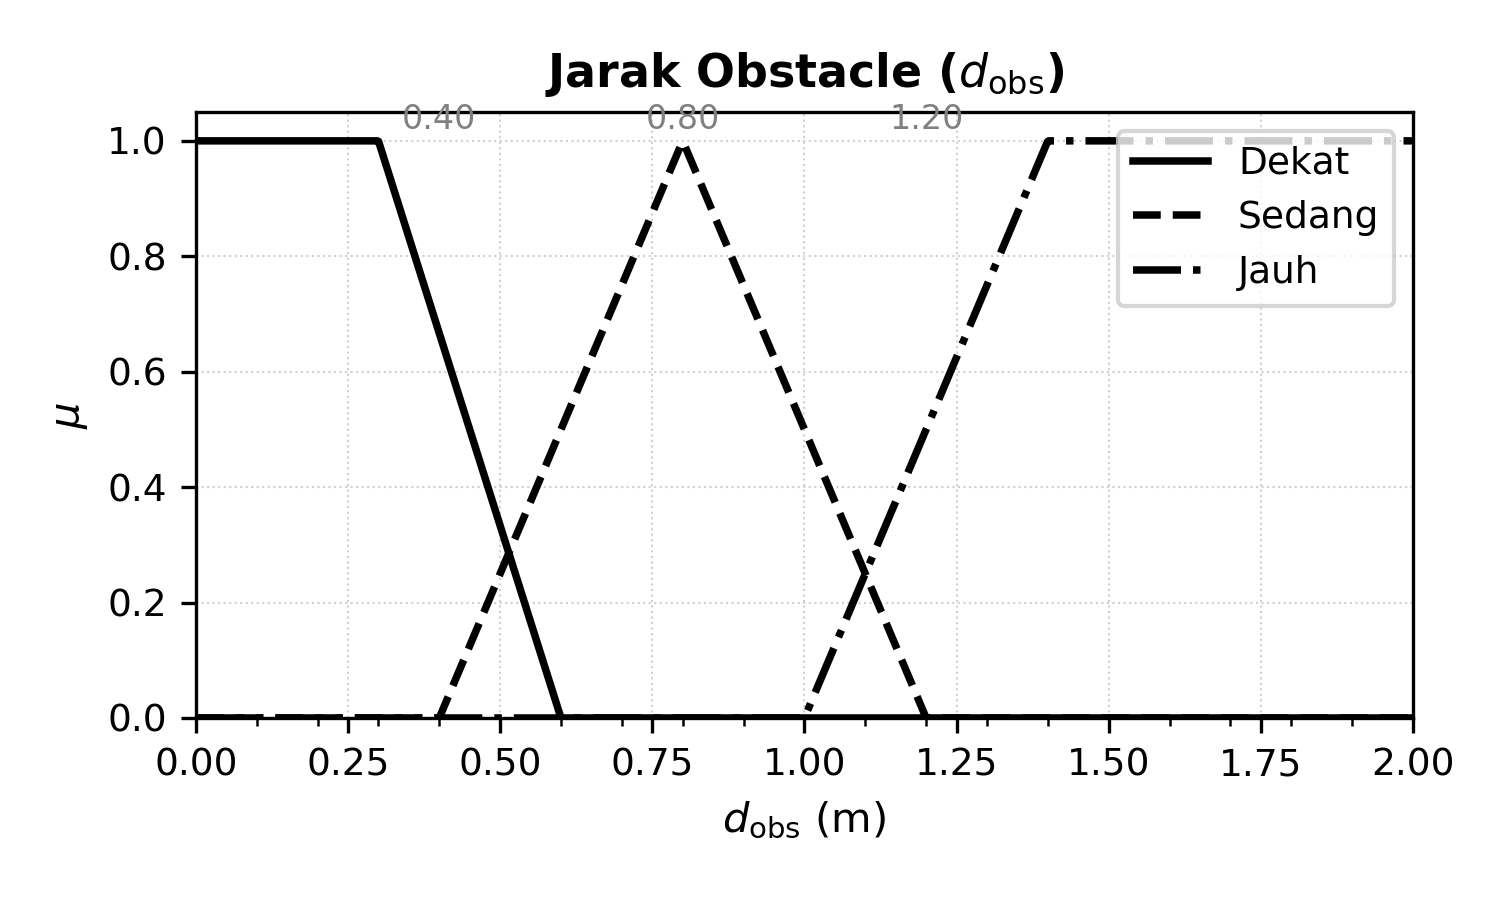
\includegraphics[width=0.48\textwidth]{gambar/3.7_fig_mf_jarak.png} %gambar/fig_mf_jarak
    \hfill
    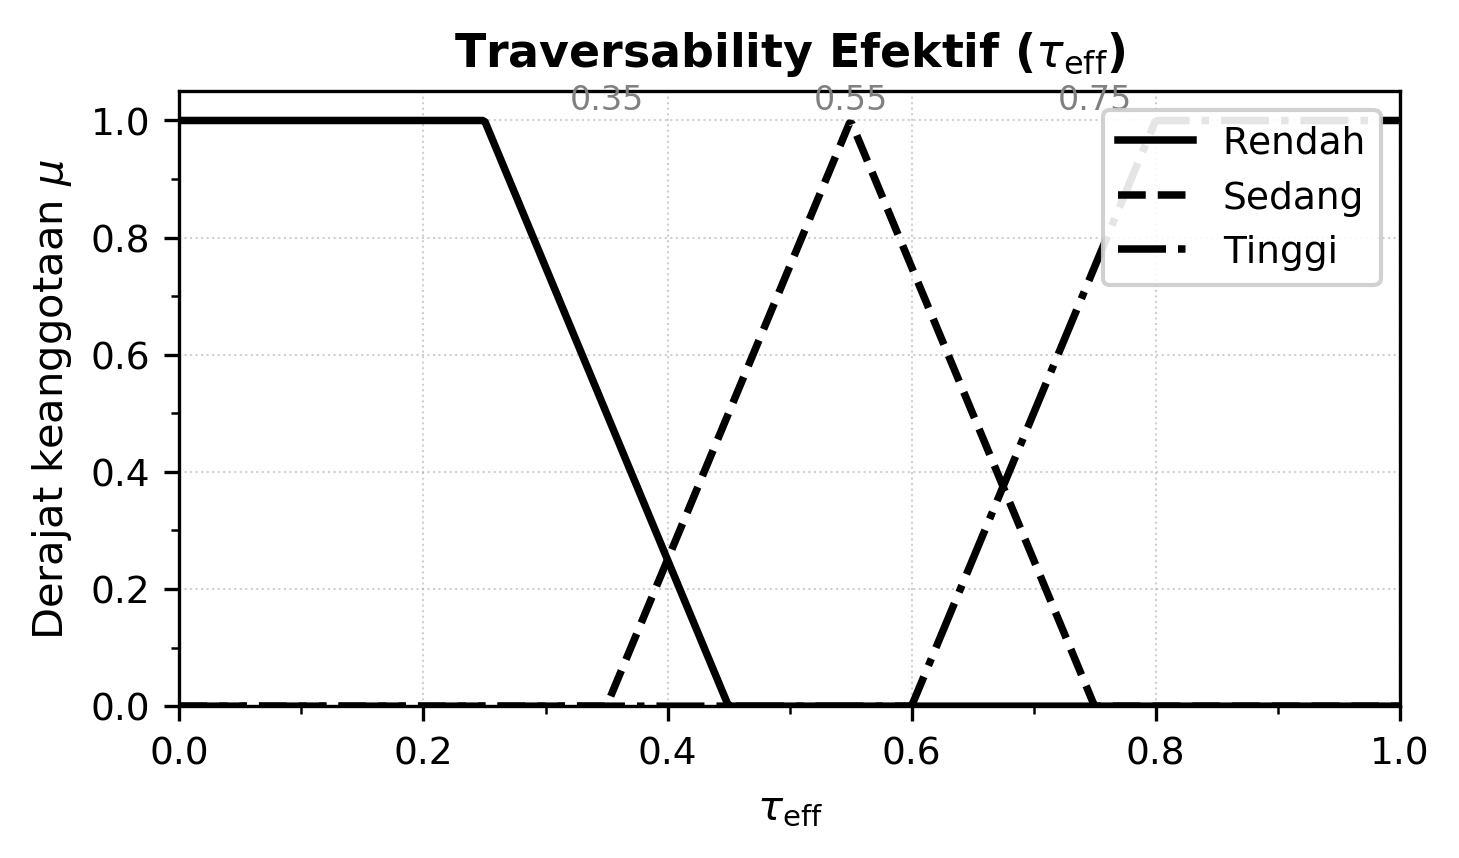
\includegraphics[width=0.48\textwidth]{gambar/3.7_fig_mf_trav.png} %gambar/fig_mf_trav
    \caption{Fungsi keanggotaan variabel input. Kiri: jarak \textit{obstacle} ($d_\text{obs}$, domain $[0, 2]$~m). Kanan: \textit{traversability} efektif ($\tau_\text{eff}$, domain $[0, 1]$).}
    \label{fig:mf_jarak}
\end{figure}

\begin{figure}[H]
    \centering
    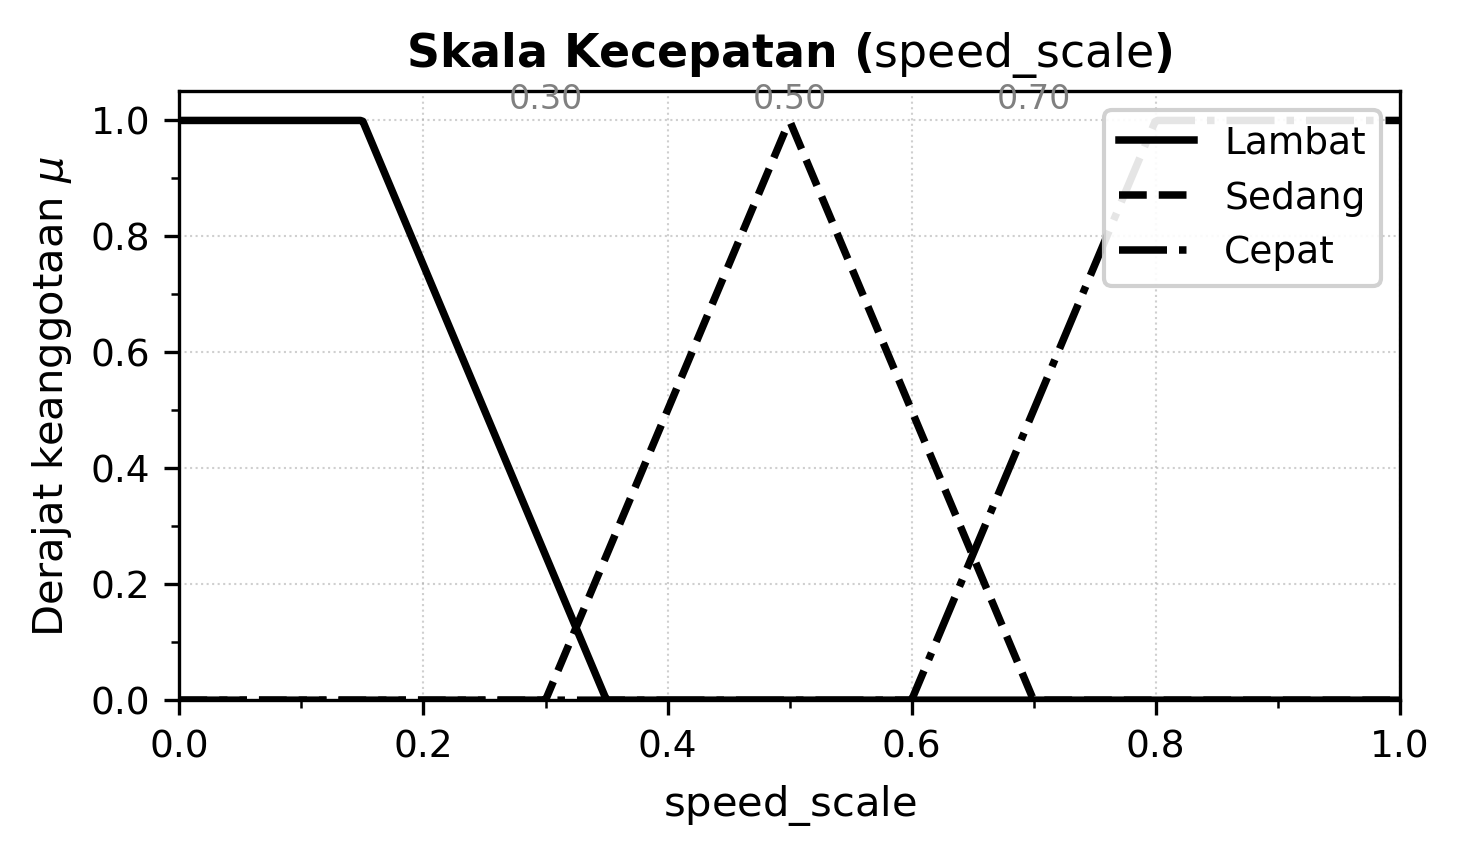
\includegraphics[width=0.48\textwidth]{gambar/3.7_fig_mf_kecepatan.png} %gambar/fig_mf_kecepatan
    \hfill
    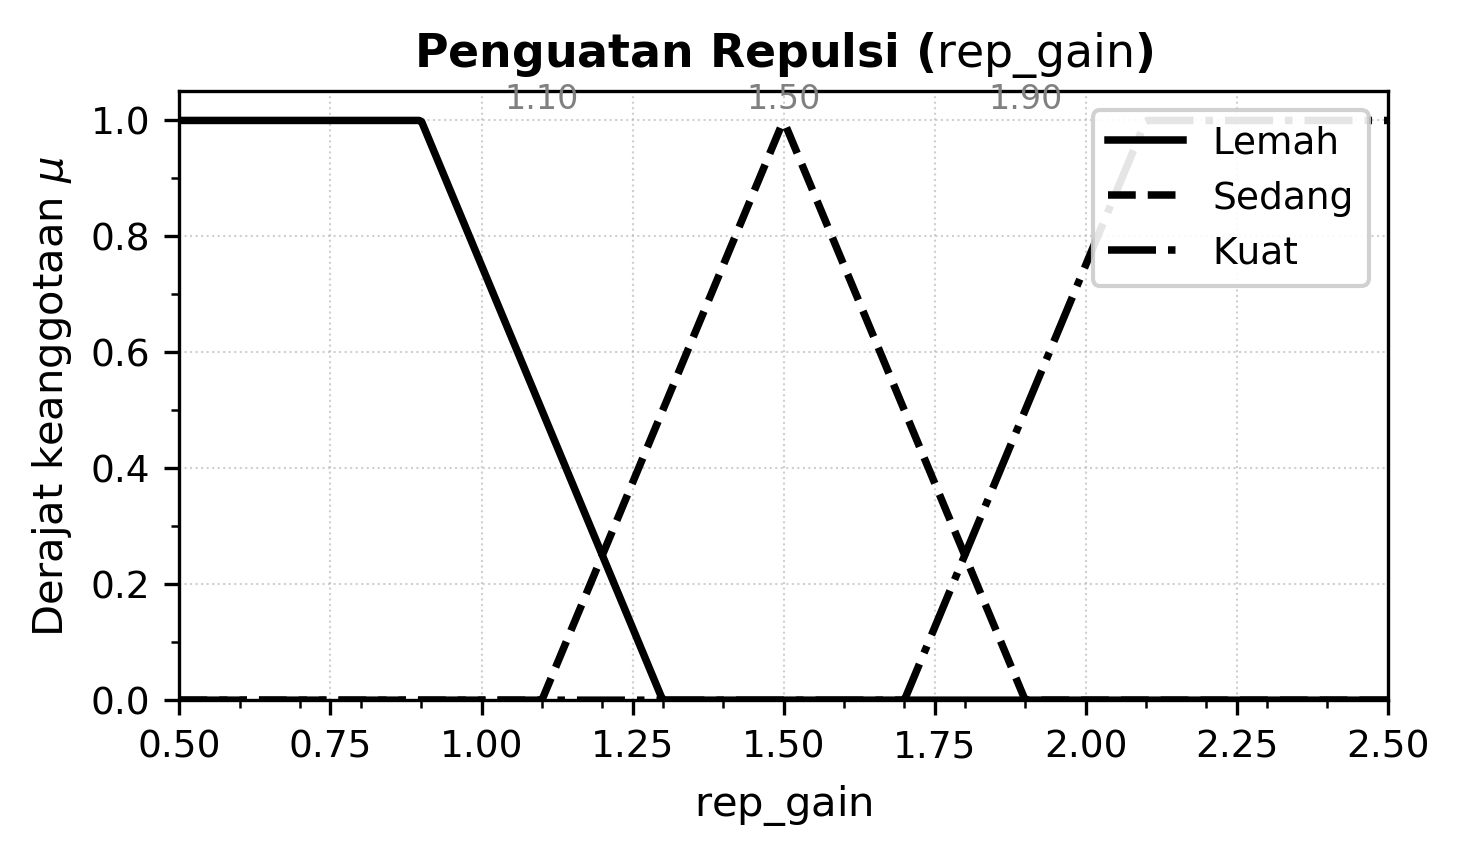
\includegraphics[width=0.48\textwidth]{gambar/3.7_fig_mf_gain.png} %gambar/fig_mf_gain
    \caption{Fungsi keanggotaan variabel output. Kiri: skala kecepatan (\textit{speed\_scale}, domain $[0, 1]$). Kanan: penguatan repulsi (\textit{rep\_gain}, domain $[0{,}5, 2{,}5]$).}
    \label{fig:mf_gain}
\end{figure}

\subsection{Basis Aturan Fuzzy}
\label{sec:basis_aturan}

Hubungan antara variabel masukan dan keluaran direpresentasikan menggunakan sembilan aturan fuzzy Mamdani. Aturan tersebut dirancang berdasarkan prinsip dasar navigasi robot bergerak, yaitu memperlambat robot dan memperbesar gaya tolak ketika obstacle semakin dekat atau traversability lingkungan menurun.

Tabel~\ref{tab:rule_base} menunjukkan basis aturan yang digunakan.

\begin{table}[H]
\centering
\caption{Basis aturan fuzzy Mamdani}
\label{tab:rule_base}
\begin{tabular}{cccc}
\toprule
\multirow{2}{*}{$d_{obs}$}
&
\multicolumn{3}{c}{$\tau_{eff}$}
\\
\cmidrule(lr){2-4}
&
Low &
Medium &
High
\\
\midrule
Near
&
Slow, Strong
&
Slow, Strong
&
Medium, Strong
\\

Medium
&
Slow, Strong
&
Medium, Medium
&
Fast, Medium
\\

Far
&
Medium, Medium
&
Fast, Weak
&
Fast, Weak
\\
\bottomrule
\end{tabular}
\end{table}

Aturan fuzzy yang digunakan dapat dituliskan sebagai berikut:

\begin{enumerate}
\item IF $d_{obs}$ is Near AND $\tau_{eff}$ is Low THEN Speed is Slow AND Gain is Strong.
\item IF $d_{obs}$ is Near AND $\tau_{eff}$ is Medium THEN Speed is Slow AND Gain is Strong.
\item IF $d_{obs}$ is Near AND $\tau_{eff}$ is High THEN Speed is Medium AND Gain is Strong.
\item IF $d_{obs}$ is Medium AND $\tau_{eff}$ is Low THEN Speed is Slow AND Gain is Strong.
\item IF $d_{obs}$ is Medium AND $\tau_{eff}$ is Medium THEN Speed is Medium AND Gain is Medium.
\item IF $d_{obs}$ is Medium AND $\tau_{eff}$ is High THEN Speed is Fast AND Gain is Medium.
\item IF $d_{obs}$ is Far AND $\tau_{eff}$ is Low THEN Speed is Medium AND Gain is Medium.
\item IF $d_{obs}$ is Far AND $\tau_{eff}$ is Medium THEN Speed is Fast AND Gain is Weak.
\item IF $d_{obs}$ is Far AND $\tau_{eff}$ is High THEN Speed is Fast AND Gain is Weak.
\end{enumerate}

\subsection{Inferensi dan Defuzzifikasi}

Metode inferensi yang digunakan adalah Mamdani dengan operator AND berupa minimum (\textit{minimum operator}). Kekuatan aktivasi aturan ke-$k$ dihitung menggunakan:

\begin{equation}
w_k
=
\min
\left(
\mu_A(d_{obs}),
\mu_B(\tau_{eff})
\right)
\label{eq:fuzzy_rule_strength}
\end{equation}

dengan:

\begin{itemize}
\item $w_k$ adalah kekuatan aktivasi aturan ke-$k$,
\item $\mu_A(d_{obs})$ adalah derajat keanggotaan jarak obstacle,
\item $\mu_B(\tau_{eff})$ adalah derajat keanggotaan traversability.
\end{itemize}

Seluruh keluaran aturan kemudian digabungkan menggunakan operator maksimum:

\begin{equation}
\mu_{agg}(y)
=
\max
\left(
\mu_1(y),
\mu_2(y),
\dots,
\mu_n(y)
\right)
\label{eq:fuzzy_aggregation}
\end{equation}

Tahap terakhir adalah defuzzifikasi menggunakan metode \textit{Center of Gravity} (CoG):

\begin{equation}
y^*
=
\frac
{\int y\,\mu_{agg}(y)\,dy}
{\int \mu_{agg}(y)\,dy}
\label{eq:fuzzy_centroid}
\end{equation}

dengan $y^*$ merupakan nilai crisp keluaran fuzzy.

Melalui proses tersebut diperoleh nilai \textit{Speed Scale} dan \textit{Repulsive Gain} yang digunakan untuk menyesuaikan perilaku navigasi robot.

\subsection{Integrasi Fuzzy dengan APFPlanner}

Nilai \textit{Speed Scale} dan \textit{Repulsive Gain} yang dihasilkan oleh sistem fuzzy digunakan untuk memodifikasi parameter APFPlanner secara \textit{real-time}.

Kecepatan linear robot dihitung menggunakan:

\begin{equation}
v
=
S
\cdot
v_{base}
\label{eq:fuzzy_speed_scale}
\end{equation}

dengan:

\begin{itemize}
\item $v$ adalah kecepatan linear aktual robot,
\item $v_{base}$ adalah kecepatan dasar APF,
\item $S$ adalah keluaran \textit{Speed Scale}.
\end{itemize}

Sementara itu, gaya tolak APF dimodifikasi menggunakan:

\begin{equation}
F_{rep}
=
G
\cdot
F_{rep}^{base}
\label{eq:fuzzy_repulsive_gain}
\end{equation}

dengan:

\begin{itemize}
\item $F_{rep}$ adalah gaya tolak setelah adaptasi,
\item $F_{rep}^{base}$ adalah gaya tolak dasar APF,
\item $G$ adalah keluaran \textit{Repulsive Gain}.
\end{itemize}

Melalui mekanisme tersebut, robot dapat bergerak lebih cepat ketika kondisi lingkungan aman dan secara otomatis memperlambat pergerakan serta meningkatkan kemampuan penghindaran obstacle ketika traversability menurun atau obstacle berada pada jarak yang dekat. Integrasi ini menghasilkan sistem \textit{Fuzzy-Adaptive Artificial Potential Field} yang lebih adaptif dibandingkan APF konvensional dengan parameter tetap.